\subsection{Voltage Divider Bias Circuit:}

\setcounter{equation}{0}

The circuit in Figure 5.1.0 it's the same that Figure 3.1.0, but this time we are going to analyze the circuit converting it first in his {\bfseries\itshape Basic Polarization} circuit, and then, proceed to make the respective calculations. \hfill

\begin{multicols}{2}
\begin{figure}[H]
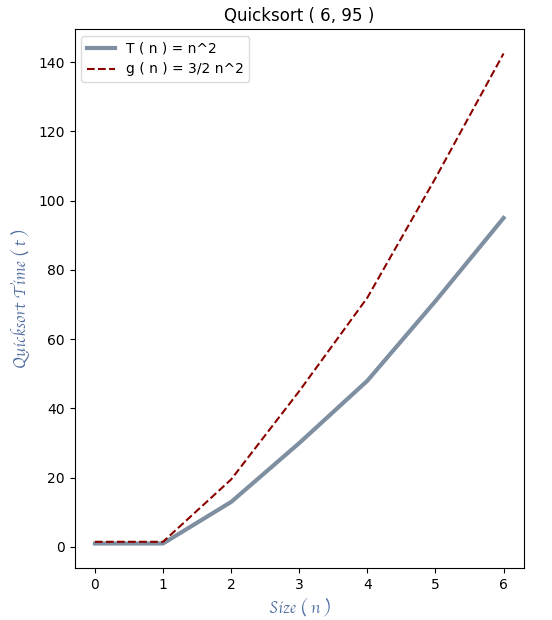
\includegraphics[width = 6cm, height = 8cm]{p1.png}
\centering \linebreak \linebreak Figure 5.1.0: Voltage divider bias circuit.
\end{figure}

\begin{figure}[H]
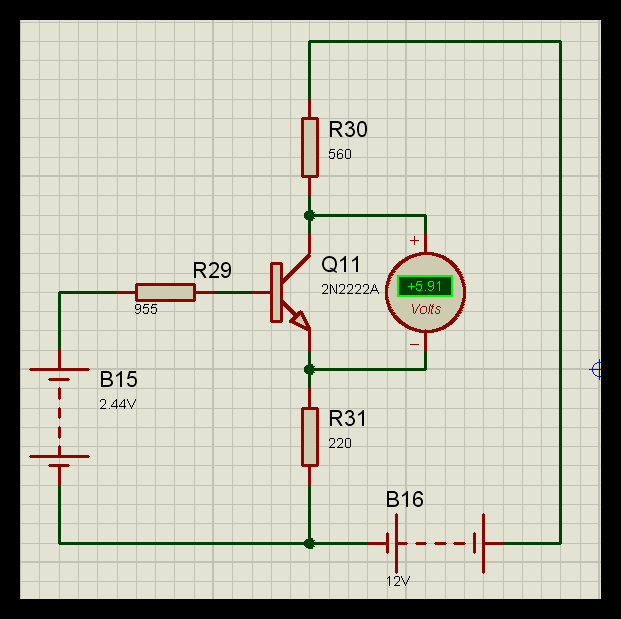
\includegraphics[width = 6cm, height = 8cm]{Equivalent1.png}
\centering \linebreak \linebreak Figure 5.1.1: Equivalent basic polarization circuit.
\end{figure}
\end{multicols} \hfill

{\bfseries
\begin{itemize}
\item First circuit parameters:
\begin{tasks}
\task $V_{BE} =  0.7 V$
\task $R_{1} = 4700 \Omega$
\task $R_{2} = 1200 \Omega$
\task $R_{C} = 560 \Omega$
\task $R_{E} = 220 \Omega$
\task $\beta = 242 $
\end{tasks}
\end{itemize}} \hfill \break

{\bfseries\itshape\color{Violet}{
\begin{itemize}
\item For $R_{B}:$
\end{itemize}}} 

\begin{flushright}
{\bfseries\itshape\color{carmine}{Formula: $R_{B}\ =\ \frac{(\ R_{1}\ )\ (\ R_{2}\ )}{R_{1}\ +\ R_{2}}:$}} \hfill \break
\end{flushright}

\begin{ceqn}
\begin{align}
R_{B}\ &=\ \frac{(\ 4700\ \Omega\ )\ (\ 1200\ \Omega\ )}{1200\ \Omega\ +\ 4700\ \Omega\ } \\ \\
&=\ 955.9\ \Omega
\end{align}
\end{ceqn} \pagebreak

{\bfseries\itshape\color{Violet}{
\begin{itemize}
\item For $E_{B}:$
\end{itemize}}} 

\begin{flushright}
{\bfseries\itshape\color{carmine}{Formula: $E_{B}\ =\ \frac{(\ E_{C}\ )\ (\ R_{2}\ )}{R_{1}\ +\ R_{2}}:$}} \hfill \break
\end{flushright}

\begin{ceqn}
\begin{align}
R_{B}\ &=\ \frac{(\ 12\ V\ )\ (\ 1200\ \Omega\ )}{1200\ \Omega\ +\ 4700\ \Omega\ } \\ \\
&=\ 2.44\ V
\end{align}
\end{ceqn} \hfill \break

{\bfseries\itshape\color{Violet}{
\begin{itemize}
\item For $I_{B}:$
\end{itemize}}} 

\begin{flushright}
{\bfseries\itshape\color{carmine}{Formula: $E_{B}\ =\ \frac{E_{B}\ -\ V_{BE}}{R_{B}\ +\ (\ \beta\ +\ 1\ )\ R_{E}}:$}} \hfill \break
\end{flushright} 

\begin{ceqn}
\begin{align}
E_{B}\ &=\ \frac{2.44\ V\ -\ 0.7\ V}{955.9\ \Omega\ +\ (\ 243\ )\ (\ 220\ \Omega\ )} \\ \\
&=\ 3 \mu A
\end{align}
\end{ceqn} 

{\bfseries\itshape\color{Violet}{
\begin{itemize}
\item For $I_{C}:$
\end{itemize}}} 

\begin{flushright}
{\bfseries\itshape\color{carmine}{Formula: $I_{C}\ =\ (\ \beta\ )\ I_{B}:$}} \hfill \break
\end{flushright}

\begin{ceqn}
\begin{align}
I_{C}\ &=\ (\ 242\ )\ (\ 3\ \mu A\ ) \\ \\
&=\ 7.7\ mA
\end{align}
\end{ceqn} \hfill \break

{\bfseries\itshape\color{Violet}{
\begin{itemize}
\item For $V_{CE}:$
\end{itemize}}}

\begin{flushright}
{\bfseries\itshape\color{carmine}{Formula: $V_{CE}\ =\ E_{C}\ -\ I_{C}\ (\ R_{C}\ +\ R_{E}\ ):$}} \hfill \break
\end{flushright}

\begin{ceqn}
\begin{align}
V_{CE}\ &=\ 12\ V\ -\ 7.7\ mA\ (\ 560\ \Omega\ +\ 220\ \Omega\ ) \\ \\
&= 5.9 V
\end{align}
\end{ceqn} \hfill \break

{\bfseries\itshape\color{Violet}{
\begin{itemize}
\item For $V_{E}:$
\end{itemize}}}

\begin{flushright}
{\bfseries\itshape\color{carmine}{Formula: $V_{E}\ =\ I_{C}\ R_{E}:$}} \hfill \break
\end{flushright}

\begin{ceqn}
\begin{align}
V_{E}\ &=\ (\ 7.7\ mA\ )\ (\ 220\ \Omega\ ) \\ \\
&=\ 1.6\ V
\end{align}
\end{ceqn} \hfill \break

{\bfseries\itshape\color{Violet}{
\begin{itemize}
\item For $V_{B}:$
\end{itemize}}} 

\begin{flushright}
{\bfseries\itshape\color{carmine}{Formula: $V_{B}\ =\ V_{BE}\ +\ V_{E}:$}} \hfill \break
\end{flushright}

\begin{ceqn}
\begin{align}
V_{B}\ &=\ 0.7\ V\ +\ 1.6\ V \\ \\
&=\ 2.3\ V
\end{align}
\end{ceqn} 

\pagebreak

The same process previously performed for "converting" the divider bias circuit, into the basic polarization one, it's executed bellow. The difference for the rest of the calculations it's that this time we are contemplating a {\bfseries\itshape BC547} transistor.

\begin{multicols}{2}
\begin{figure}[H]
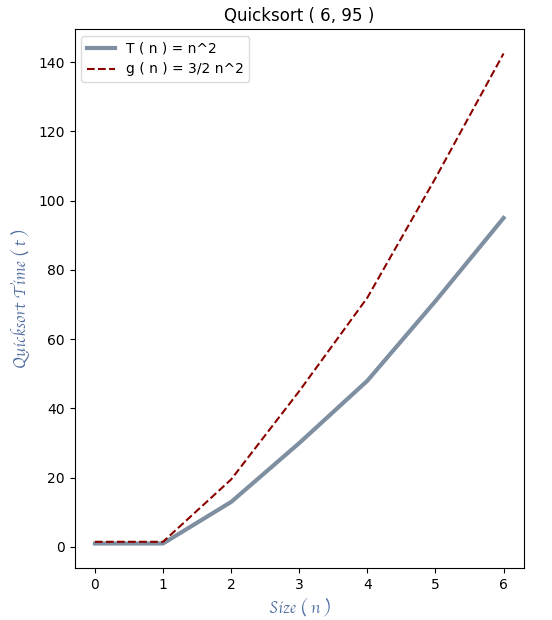
\includegraphics[width = 6cm, height = 8cm]{p1.png}
\centering \linebreak \linebreak Figure 5.1.2: Voltage divider bias circuit.
\end{figure}

\begin{figure}[H]
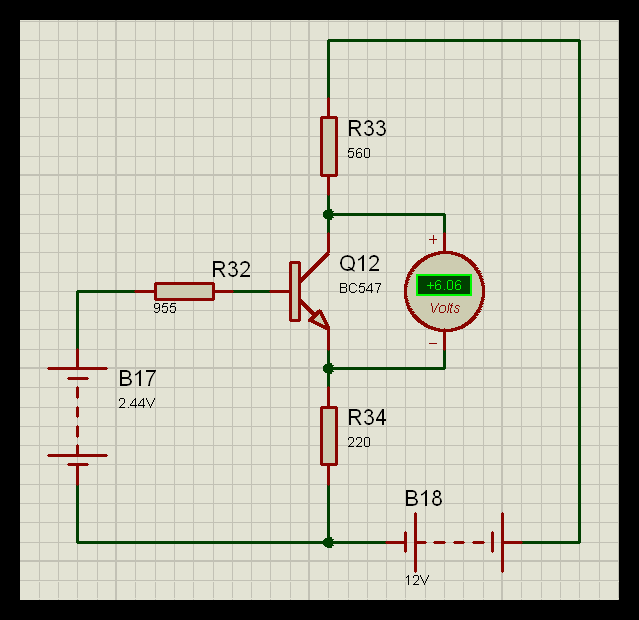
\includegraphics[width = 6cm, height = 8cm]{Equivalent2.png}
\centering \linebreak \linebreak Figure 5.1.3: Equivalent basic polarization circuit.
\end{figure}
\end{multicols} \hfill

\setcounter{equation}{0}

{\bfseries
\begin{itemize}
\item Second circuit parameters:
\begin{tasks}
\task $V_{BE} =  0.7 V$
\task $R_{1} = 4700 \Omega$
\task $R_{2} = 1200 \Omega$
\task $R_{C} = 560 \Omega$
\task $R_{E} = 220 \Omega$
\task $\beta = 595 $
\end{tasks}
\end{itemize}} \hfill \break

{\bfseries\itshape\color{Violet}{
\begin{itemize}
\item For $R_{B}:$
\end{itemize}}} 

\begin{flushright}
{\bfseries\itshape\color{carmine}{Formula: $R_{B}\ =\ \frac{(\ R_{1}\ )\ (\ R_{2}\ )}{R_{1}\ +\ R_{2}}:$}} \hfill \break
\end{flushright}

\begin{ceqn}
\begin{align}
R_{B}\ &=\ \frac{(\ 4700\ \Omega\ )\ (\ 1200\ \Omega\ )}{1200\ \Omega\ +\ 4700\ \Omega\ } \\ \\
&=\ 955.9\ \Omega
\end{align}
\end{ceqn} \pagebreak

{\bfseries\itshape\color{Violet}{
\begin{itemize}
\item For $E_{B}:$
\end{itemize}}} 

\begin{flushright}
{\bfseries\itshape\color{carmine}{Formula: $E_{B}\ =\ \frac{(\ E_{C}\ )\ (\ R_{2}\ )}{R_{1}\ +\ R_{2}}:$}} \hfill \break
\end{flushright}

\begin{ceqn}
\begin{align}
R_{B}\ &=\ \frac{(\ 12\ V\ )\ (\ 1200\ \Omega\ )}{1200\ \Omega\ +\ 4700\ \Omega\ } \\ \\
&=\ 2.44\ V
\end{align}
\end{ceqn} \hfill \break

{\bfseries\itshape\color{Violet}{
\begin{itemize}
\item For $I_{B}:$
\end{itemize}}} 

\begin{flushright}
{\bfseries\itshape\color{carmine}{Formula: $E_{B}\ =\ \frac{E_{B}\ -\ V_{BE}}{R_{B}\ +\ (\ \beta\ +\ 1\ )\ R_{E}}:$}} \hfill \break
\end{flushright}

\begin{ceqn}
\begin{align}
E_{B}\ &=\ \frac{2.44\ V\ -\ 0.7\ V}{9.55.9\ \Omega\ +\ (\ 596\ )\ (\ 220\ \Omega\ )} \\ \\
&=\ 1.3 \mu A
\end{align}
\end{ceqn} 

{\bfseries\itshape\color{Violet}{
\begin{itemize}
\item For $I_{C}:$
\end{itemize}}} 

\begin{flushright}
{\bfseries\itshape\color{carmine}{Formula: $I_{C}\ =\ (\ \beta\ )\ I_{B}:$}} \hfill \break
\end{flushright}

\begin{ceqn}
\begin{align}
I_{C}\ &=\ (\ 595\ )\ (\ 1.3\ \mu A\ ) \\ \\
&=\ 7.8\ mA
\end{align}
\end{ceqn} \hfill \break

{\bfseries\itshape\color{Violet}{
\begin{itemize}
\item For $V_{CE}:$
\end{itemize}}} 

\begin{flushright}
{\bfseries\itshape\color{carmine}{Formula: $V_{CE}\ =\ E_{C}\ -\ I_{C}\ (\ R_{C}\ +\ R_{E}\ ):$}} \hfill \break
\end{flushright}

\begin{ceqn}
\begin{align}
V_{CE}\ &=\ 12\ V\ -\ 7.8\ mA\ (\ 560\ \Omega\ +\ 220\ \Omega\ ) \\ \\
&= 5.9 V
\end{align}
\end{ceqn} \hfill \break

{\bfseries\itshape\color{Violet}{
\begin{itemize}
\item For $V_{E}:$
\end{itemize}}} 

\begin{flushright}
{\bfseries\itshape\color{carmine}{Formula: $V_{E}\ =\ I_{C}\ R_{E}:$}} \hfill \break
\end{flushright}

\begin{ceqn}
\begin{align}
V_{E}\ &=\ (\ 7.8\ mA\ )\ (\ 220\ \Omega\ ) \\ \\
&=\ 1.7\ V
\end{align}
\end{ceqn} \hfill \break

{\bfseries\itshape\color{Violet}{
\begin{itemize}
\item For $V_{B}:$
\end{itemize}}}

\begin{flushright}
{\bfseries\itshape\color{carmine}{Formula: $V_{B}\ =\ V_{BE}\ +\ V_{E}:$}} \hfill \break
\end{flushright}

\begin{ceqn}
\begin{align}
V_{B}\ &=\ 0.7\ V\ +\ 1.7\ V \\ \\
&=\ 2.4\ V
\end{align}
\end{ceqn} 

\pagebreak